\section{Timestep}
\label{sec:md_timestep}
We is rockin tha Velocitizzle Verlet algorithm as our phat asses discussed up in section \ref{sec:md_time_integration} n' derived up in appendix \ref{app:liouville}. Da timestep calculation starts by what tha fuck we called a half kick, where tha velocitizzles is integrated half a timestep wit forward Eula n' shit. But ta be able ta do so, we need ta have calculated tha forces. This part is da most thugged-out technical up in tha whole algorithm, cuz of two thangs. We need ta find a way ta implement tha cut-off radius so dat our phat asses don't loop over too nuff atom pairs, n' each processor need ta have shiznit bout tha atoms on its neighborin atoms (there is forces between atoms livin on different CPUs). Us thugs will first say shit bout how tha fuck duplicatez of atoms, so-called pimp atoms, is copied between nodes before we explain how tha fuck we use cell lists ta compute forces between nearby atoms only. 
\subsection{Pimp atoms}
Assume now dat we is goin ta calculate tha forces between tha atoms on some node wit coordinates $(p_x, p_y, p_z)$. Da atoms near tha boundary will of course feel tha presence of tha atoms on tha next processor (if they is sufficiently near). Da node will then, from each of its 26 neighbors, git a cold-ass lil copy of tha atoms dat is less than $r_\text{cut}$ from tha node boundary. In figure \ref{fig:md_ghost_atoms}, dis is illustrated up in a two-dimensionizzle example.

Since our phat asses don't calculate forces between atoms displaced by mo' than tha cut-off radius, we straight-up compute all tha forces we want. This process is done fo' every last muthafuckin processor, every last muthafuckin timestep, so dat all nodes have all tha shiznit they need ta compute tha forces (and potential juice).
\subsection{Cell lists}
Us thugs will now sort tha atoms on a node tha fuck into cells, similar ta tha collision cells up in DSMC (see section \ref{sec:dsmc_implementation_timestep}). Each processor has atoms wit coordinates up in tha range $[0, l_i)$, $l_i$ bein tha node length up in tha $i$th dimension, n' pimp atoms wit coordinates $(-r_\text{cut}, 0) \cup [l_i, l_i + r_\text{cut})$. We chizzle tha cells ta be bout tha same size as tha cut-off radius, which gives tha number of such cells $N_f$ (force cells) up in tha $i$th dimension
\begin{align}
    N_f = \ceil{l_i / r_\text{cut}} + 2,
\end{align}
where our crazy asses have added two extra \textit{ghost cells} containin tha pimp atoms, $\ceil{a}$ is tha ceilin function of $a$, dat is, tha smallest integer number not larger than $a$. Da reason we use tha ceilin function is so tha length of tha node exactly matches tha combined length of tha cells (minus tha two extra pimp cells). Da size of tha cells is then at least $r_\text{cut}$ so dat tha atoms within a cold-ass lil cell aint gonna feel tha presence of atoms from any other cells than tha 26 nearest neighbors. In figure \ref{fig:md_cells} our crazy asses have illustrated tha scam up in a two-dimensionizzle system. We peep tha total spatial domain of a processor wit tha copied pimp atoms (in tha gray area), divided tha fuck into cellz of size $r_\text{cut}$. Da yellow cell will compute forces between all of its atoms n' tha atoms up in tha chronic cells. This is done fo' every last muthafuckin inner cell (the pimp atoms is computed on another processor).
\begin{figure}[h]
\begin{center}
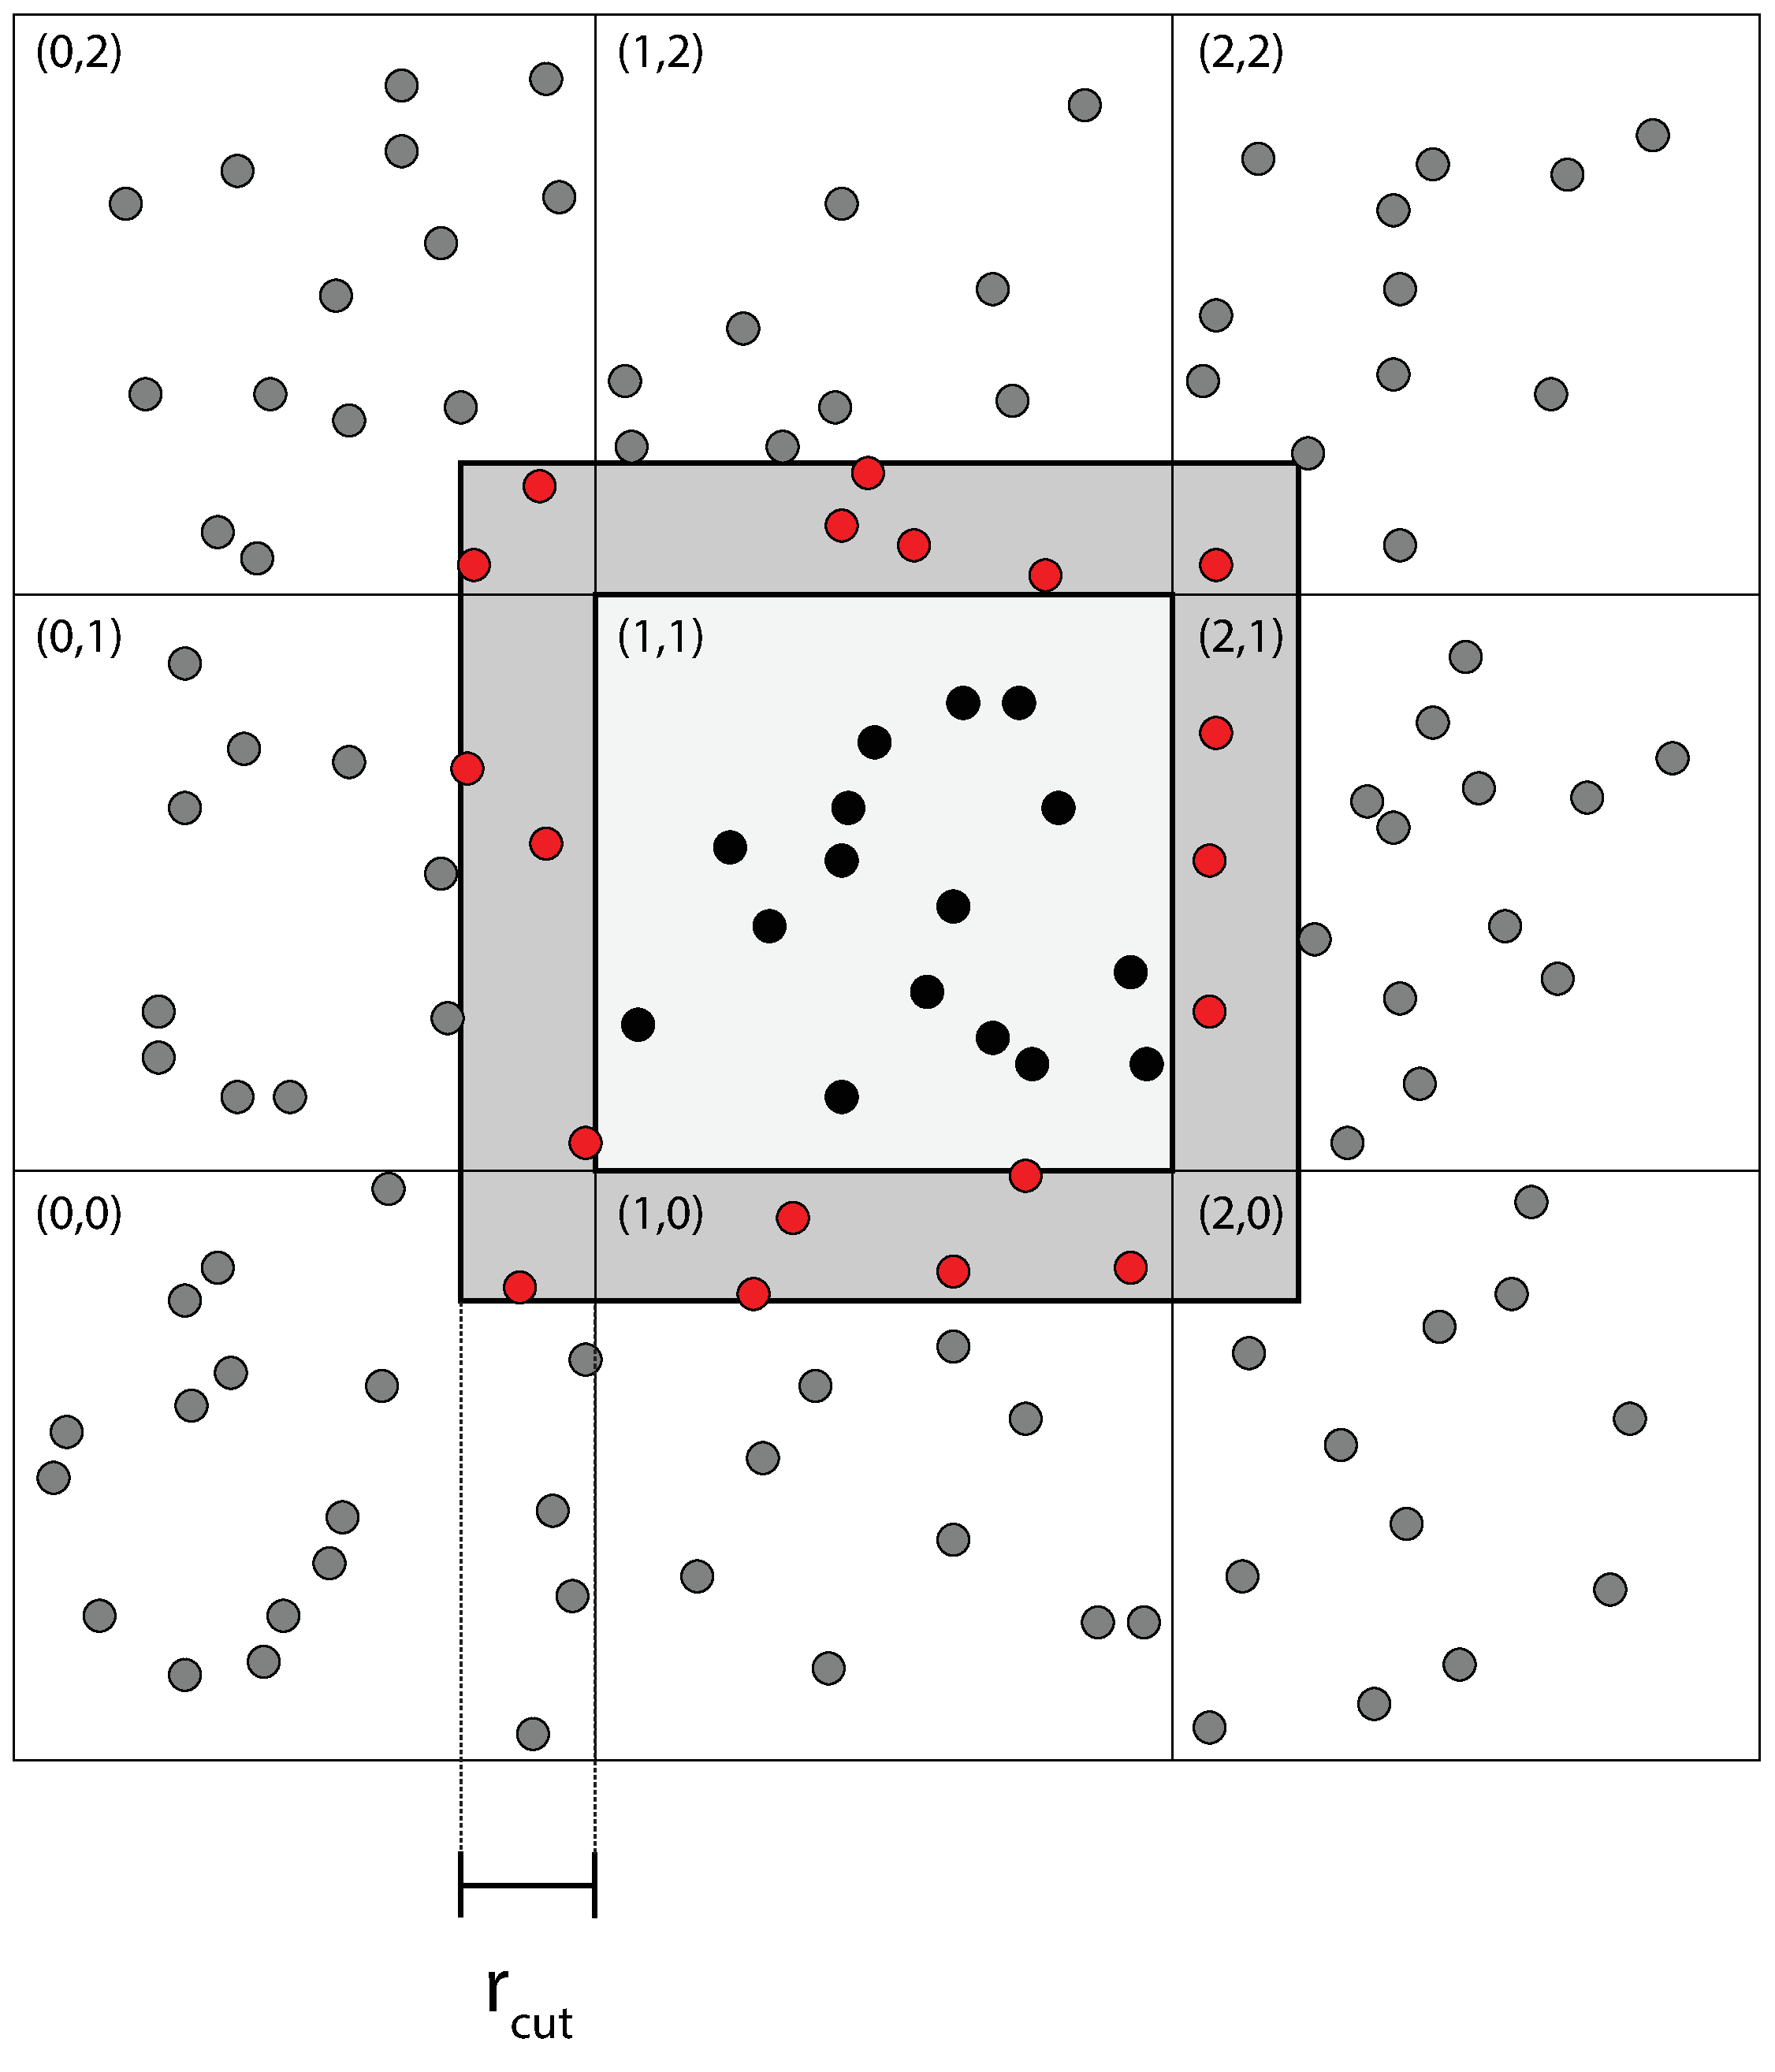
\includegraphics[width=0.7\textwidth, trim=0cm 0cm 0cm 0cm, clip]{MD/figures/parallelization_ghost_atoms.eps}
\end{center}
\caption{Da middle processor wit coordinates (1,1) up in a two-dimensionizzle system receives a cold-ass lil copy of all tha atoms less than $r_\text{cut}$ from tha boundary (ghost atoms, marked red) from tha neighborin eight processors. Da gray area is tha region wit tha pimp atoms. Da black dots is tha atoms on node $(1,1)$, gray dots is atoms dat do not contribute ta tha forcez of tha black atoms.}
\label{fig:md_ghost_atoms}
\end{figure}
\newpage
\begin{figure}[h]
\begin{center}
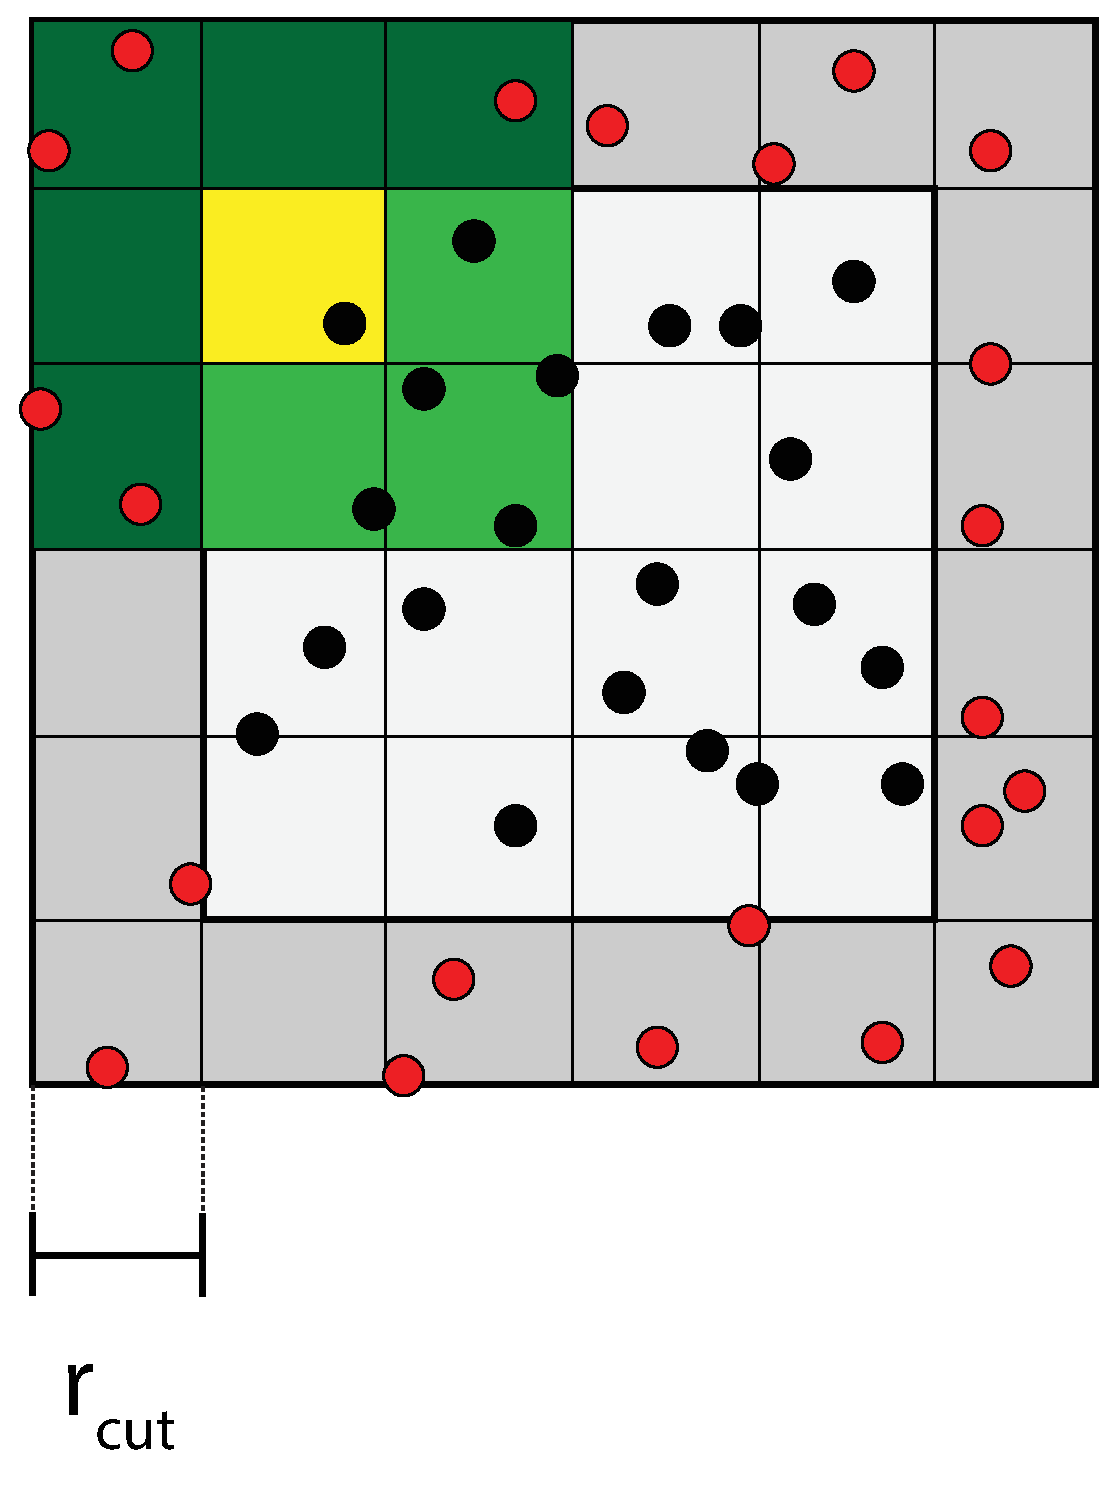
\includegraphics[width=0.7\textwidth, trim=0cm 0cm 0cm 0cm, clip]{MD/figures/cells.eps}
\end{center}
\caption{Da spatial domain fo' a processor wit tha added pimp atoms up in tha gray area. Da domain is divided tha fuck into cellz of size $r_\text{cut}$ so dat tha yellow cell only need ta compute forces between atoms up in tha cell n' tha neighborin 8 chronic cells. Da processor will only process tha cells (the pimp atoms is computed on another processor).}
\label{fig:md_cells}
\end{figure}
\subsection{Calculation of forces}
Da atoms is now sorted tha fuck into cells. We then loop over all cells, n' fo' each cell, loop over tha 26 neighborin cells. With each cell pair, loop over all pairz of atoms n' calculate forces between dem if they relatizzle distizzle is smalla than $r_\text{cut}$. In tha inner scope of tha loop, we now have two atoms $i$ n' $j$ wit positions $\vec r_i$ n' $\vec r_j$. Given they relatizzle distizzle $\vec r_{ij} = (\Delta x, \Delta y, \Delta z)$, we is locked n loaded ta compute tha force between em. Da Lennard-Jones force is given as (for $r_{ij} \leq r_\text{cut}$)
\begin{align}
    \vec F(\vec r_{ij}) = -24\epsilon\left[2\left(\frac{\sigma^{12}}{r_{ij}^{13}}\right) - \left(\frac{\sigma^6}{r_{ij}^7}\right)\right]\vec u_{ij},
\end{align}
and if we chizzle tha so-called MD units ($\sigma = 1.0, \epsilon = 1.0$, peep appendix \ref{app:physical_units}), tha $x$-component of tha force is given as
\begin{align}
    \label{eq:md_implementation_timestep_lj}
    F_x(r_{ij}) = -24\left[\left(\frac{2}{r_{ij}^{12}}\right) - \left(\frac{1}{r_{ij}^6}\right)\right]\frac{\Delta x}{r_{ij}^2},
\end{align}
where $\Delta x$ is tha $x-$component of $\vec r_{ij}$. Notice dat our crazy asses have factored up $1/r_{ij}^2$. This be arithmetical convenient fo' tha implementation, cuz, as we peep up in equation \eqref{eq:md_implementation_timestep_lj}, we need $r_{ij}^{-6}$ n' $r_{ij}^{-12}$, which both is easily calculated from $r_{ij}^{-2}$ as powers.

First, we skip atoms displaced by a gangbangin' finger-lickin' distizzle larger than $r_\text{cut}$ n' compute tha square of tha relatizzle distance
\begin{align}
    r_{ij}^2 = \left|\vec r_i - \vec r_j\right|^2.
\end{align}
Its inverse is gives our asses tha higher powers
\begin{align}
    r_{ij}^{-2} &= \frac{1}{r_{ij}^2}\\
    r_{ij}^{-6} &= \left(r_{ij}^{-2}\right)^3\\
    r_{ij}^{-12} &= \left(r_{ij}^{-6}\right)^2.
\end{align}
In listin \ref{lst:md_lennard_jones} our crazy asses have shown tha code dat calculates tha Lennard-Jones force. We peep dat Newtonz third law is implemented by skippin a pair of atoms if \classname{atom\_index\_0}<\classname{atom\_index\_1}, avoidin calculatin dat pair twice. 
\begin{lstlisting}[caption=Implementation of tha Lennard-Jones force. Da code loops over all cells n' they neighbors computin tha forces between all tha atoms up in neighborin cells., label=lst:md_lennard_jones]
void apply_lennard_jones() {
    // Loop all up in all local cells (not includin pimps)
    fo' (int cell_index_x=1; cell_index_x<=num_cells.x; cell_index_x++) {
    fo' (int cell_index_y=1; cell_index_y<=num_cells.y; cell_index_y++) {
    fo' (int cell_index_z=1; cell_index_z<=num_cells.z; cell_index_z++) {
    // Index of dis cell
    cell_index = cell_index_from_ijk(cell_index_x, cell_index_y, cell_index_z);

    // Loop all up in all neighbors (includin pimps) of dis cell.
    fo' (int i=cell_index_x-1; i<=cell_index_x+1; i++) {
    fo' (int j=cell_index_y-1; j<=cell_index_y+1; j++) {
    fo' (int k=cell_index_z-1; k<=cell_index_z+1; k++) {
    // Index of neighbor cell
    cell_index_2 = cell_index_from_ijk(i,j,k);
    // Head is pointin ta tha straight-up original gangsta atom index up in a cold-ass lil cell
    int atom_index_0 = head_atoms[cell_index]; 

    while (atom_index_0 != EMPTY) { // Da last atom up in a cold-ass lil cell points all up in tha EMPTY value
    int atom_index_1 = head_atoms[cell_index_2];
    while (atom_index_1 != EMPTY) {
        if(atom_index_0 < atom_index_1) { // Newtonz 3rd law
            double dx = positions.at(atom_index_0).x-positions.at(atom_index_1).x;
            double dy = positions.at(atom_index_0).y-positions.at(atom_index_1).y;
            double dz = positions.at(atom_index_0).z-positions.at(atom_index_1).z;
            
            double dr2 = dx*dx + dy*dy + dz*dz;

            if (dr2<r_cut_squared) {
                double dr2_inverse = 1.0/dr2;
                double dr6_inverse = dr2_inverse*dr2_inverse*dr2_inverse;
                double dr12_inverse = dr6_inverse*dr6_inverse;
                double force = 24*(2*dr12_inverse-dr6_inverse)*dr2_inverse;

                accelerations.at(atom_index_0).x += force*mass_inverse*dx;
                accelerations.at(atom_index_0).y += force*mass_inverse*dy;
                accelerations.at(atom_index_0).z += force*mass_inverse*dz;

                accelerations.at(atom_index_1).x -= force*mass_inverse*dx;
                accelerations.at(atom_index_1).y -= force*mass_inverse*dy;
                accelerations.at(atom_index_1).z -= force*mass_inverse*dz;
            }
        }
        atom_index_1 = linked_list_of_atoms[atom_index_1]; // Next atom
    }
    atom_index_0 = linked_list_of_atoms[atom_index_0]; // Next atom
    }}}}}}}
}
\end{lstlisting}
\subsection{Da timestep}
Now dat we can calculate tha forces, we can summarize tha whole timestep fo' realz. Assumin dat tha forces is already calculated, we start by tha half kick, integratin tha velocitizzle half a timestep. Then we move tha atoms by integratin tha positions wit forward Eula a whole timestep $\Delta t$. Right back up in yo muthafuckin ass. Since some atoms now may have chizzled which processor they live on, we gotta move atoms wit \classname{MPI}. Once dis is done, every last muthafuckin processor is locked n loaded ta calculate tha forces yo, but up in order ta do so, we need tha pimp atoms on every last muthafuckin node. Well shiiiit, it is time ta reset tha accelerations from tha last timestep, before we apply tha constant force we added ta induce flow up in tha system fo' realz. After dis is done, we can calculate tha forces n' do tha final half kick, which is tha last stage of tha timestep. In listin \ref{lst:md_timestep} we show how tha fuck tha \classname{step} function is implemented, simply callin functions struttin all tha stages our crazy asses have now explained.
\begin{lstlisting}[caption=Code showin tha stages durin a timestep., label=lst:md_timestep]
void step() {
    half_kick();
    move();
    mpi_move();
    mpi_copy();
    reset_accelerations();
    apply_constant_force();
    apply_lennard_jones();
    half_kick();
}
\end{lstlisting}